\documentclass[a4paper,11pt]{article}
\input{/home/tof/Documents/Cozy/latex-include/preambule_doc.tex}
\input{/home/tof/Documents/Cozy/latex-include/preambule_commun.tex}
\newcommand{\showprof}{show them}  % comment this line if you don't want to see todo environment
\setlength{\fboxrule}{0.8pt}
\fancyhead[L]{\fbox{\Large{\textbf{ResSoc 03}}}}
\fancyhead[C]{\textbf{Débat réseaux sociaux}}
\newdate{madate}{10}{09}{2020}
%\fancyhead[R]{\displaydate{madate}} %\today
\fancyhead[R]{Seconde - SNT}
%\fancyhead[R]{Première - NSI}
%\fancyhead[R]{Terminale - NSI}
\fancyfoot[L]{\vspace{1mm}Christophe Viroulaud}
\AtEndDocument{\label{lastpage}}
\fancyfoot[C]{\textbf{Page \thepage/\pageref{lastpage}}}
\fancyfoot[R]{\includegraphics[width=2cm,align=t]{/home/tof/Documents/Cozy/latex-include/cc.png}}

\begin{document}
Les conditions sanitaires nous obligent à organiser le débat sur les réseaux sociaux autrement. Nous allons utiliser l'application \textbf{Mur collaboratif} présente sur le lycée connecté. Vous avez accès à une carte mentale qui se nomme par exemple: \emph{débat Snapchat}. De plus, j'ai affecté (au hasard) chacun d'entre vous à un groupe \emph{pour ou contre} (voir mail).\\
Durant la semaine vous devez compléter le mur en ajoutant vos arguments à l'aide d'un post-it. Pour créer un post-it il suffit de double-cliquer où vous voulez sur le mur. Il est possible de le déplacer ensuite. Le contenu peut-être ajouté sous forme écrite, audio ou vidéo.
\begin{center}
\centering
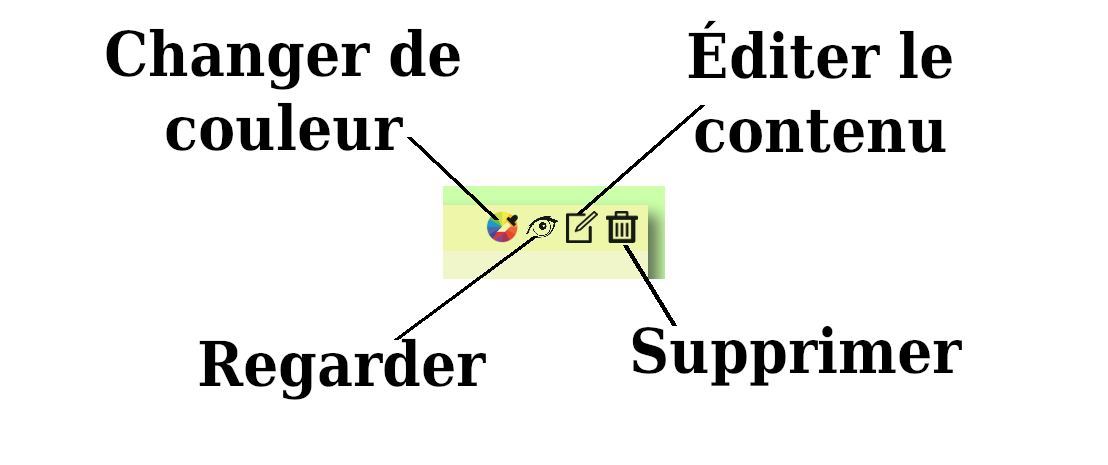
\includegraphics[width=10cm]{ressources/post-it.png}
\captionof{figure}{Modifier un post-it}
\label{postit}
\end{center}
Soyez attentif aux arguments de l'équipe adverse afin de donner une contre-argumentation efficace. Vous pouvez déplacer vos post-it pour les mettre en face des arguments adverses.

\textbf{Il est bien entendu interdit de supprimer les informations adverses. J'effectuerai un contrôle régulier des contenus et connexions.}

À la fin de la semaine je mettrai une note sur le travail effectué. Elle prendra en compte:
\begin{itemize}
    \item le travail déjà effectué par certains et envoyé par mail (bonus pour ceux qui ont fait cet effort),
    \item le contenu de la rédaction (ou présentation audio/vidéo) des arguments,
    \item les efforts de présentation (texte ou audio/vidéo),
    \item la pertinence des contre-argumentations.
\end{itemize}

Vous pouvez me contacter par mail en cas de soucis techniques.
\end{document}